\chapter{Temperature dependent chain rigidity study of organic photovoltaic donor-acceptor co-polymers.}
The following chapter contains yet to be published work written by me with the guidance of Dr. Eric Jankowski. 
\label{chap:PersistenceLength}
\section{Summary} 
Donor-acceptor (DA) co-polymers are currently a interesting area of study because of their promise in improving the field of optoelectronics because of their tunable band gaps. Applying these polymers in photovoltaic devices has proven to increase the power conversion efficiency of the device. In this study, we implemented molecular dynamics simulations to investigate the rigidity of complex organic polymers. Utilizing the previously validated workflow (Chapter 4) we built and parameterized 13 conjugated, organic polymers and predicted the bulk morphologies over a large temperature range. From the morphologies we employed a new function to calculated the persistence length $l_p^{MD}$ of each polymer throughout their trajectories. We compare the results to experimental persistence lengths calculated via small angle neutron scattering, $l_p^{SANS}$, and to theoretical results calculated via density functional theory, $l_p^{DFT}$ . We found that for most of the polymers there was good agreements between the $l_p^{MD}$ and $l_p^{SANS}$. From this information we are able to draw conclusions about how differences in side chains and backbone chemistry effects the rigidity of DA co-polymers. 
\section{Introduction}
\begin{wrapfigure}{r}{0.5\textwidth}
    \begin{center}
        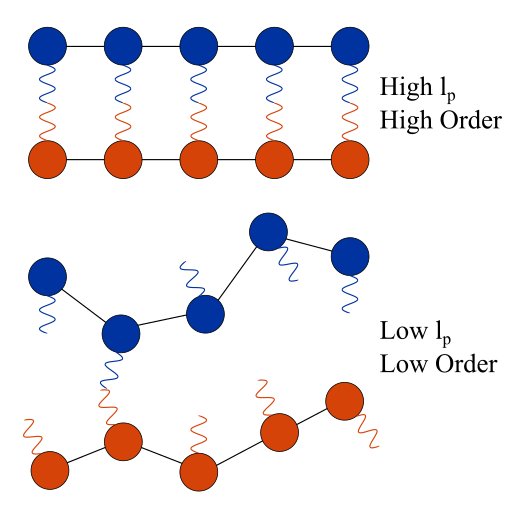
\includegraphics[width=0.48\textwidth]{src/figures/pers_l_figs/persistence_length.png}
    \end{center}    
  \caption{Diagram of how a more rigid polymer (high $l_p$) can lead to higher order in the morphology compared to a more flexible polymer (low $l_p$).}
  \label{pers_length}
\end{wrapfigure}
The morphology that OPV polymers self-assemble into has a significant impact on the power conversion efficiency (PCE) of the solar devices that are made from these materials. Currently,  there is some ambiguity as to why certain morphologies lead to an increase in the PCE as well as what materials might self-assemble into these more efficient morphologies. Drawing connections between the physical and/or chemical properties of polymers to higher efficiency morphologies will enable the discovery of new materials that could increase the PCE of OPV devices. Donor-acceptor (DA) polymers are of a great interest in OPV device design due to their tunable band-gaps and high charge carrier mobilities \citep{sarap_electronic_2023}. DA polymers function as both the electron donor and electron acceptor by alternating electron rich and electron deficient environments. DA polymers are so exciting because we can in theory tune their optoelectronic properties by altering the donors and acceptors as well as their sequencing, all while determining the thermodynamic stability using MD simulations. The persistence length ($l_p$) of a polymer is used to describe the polymer's rigidness, a smaller $l_p$ correlates to a more flexible polymer. The $l_p$ is one measure of both thermodynamic stability as well as a prediction of how well the polymer might order in a bulk morphology. The $l_p$ is a characteristic of polymer chains in a given environment that gives a lot of insight into how the polymer(s) interact and self-assemble into given morphologies. In some cases, the higher the persistence length of a polymer, the higher the observed order of the polymer bulk-morphology will be \citep{martin_temperature-dependence_2018}. Previous studies have found that the straighter a polymer with optoelectronic properties is, the greater the probability of $\pi$-stacking of the backbones, leading to a greater charge carrier mobility in the bulk morphology \citep{Himmelberger_Salleo_2015}. Danielsen et al.~ has drawn a connection between the rigidity of DA copolymers and their molecular structure and side chain size via small angle neutron scattering (SANS). With the abundance of possible donors and acceptors and infinite possible combinations it is impossible to experimentally synthesize and test many DA polymers. Due to this we turn toward molecular dynamics simulations. In this study, we present a computational workflow of modeling and predicting the persistence length of DA polymers. We validate this workflow with 13 OPV polymers by comparing the persistence lengths calculated via MD ($l_p^{MD}$) to those presented by Danielsen, et al.~ using DFT ($l_p^{DFT}$) and SANS ($l_p^{SANS}$). 

\newpage
\begin{figure}[h!]
    \centering
    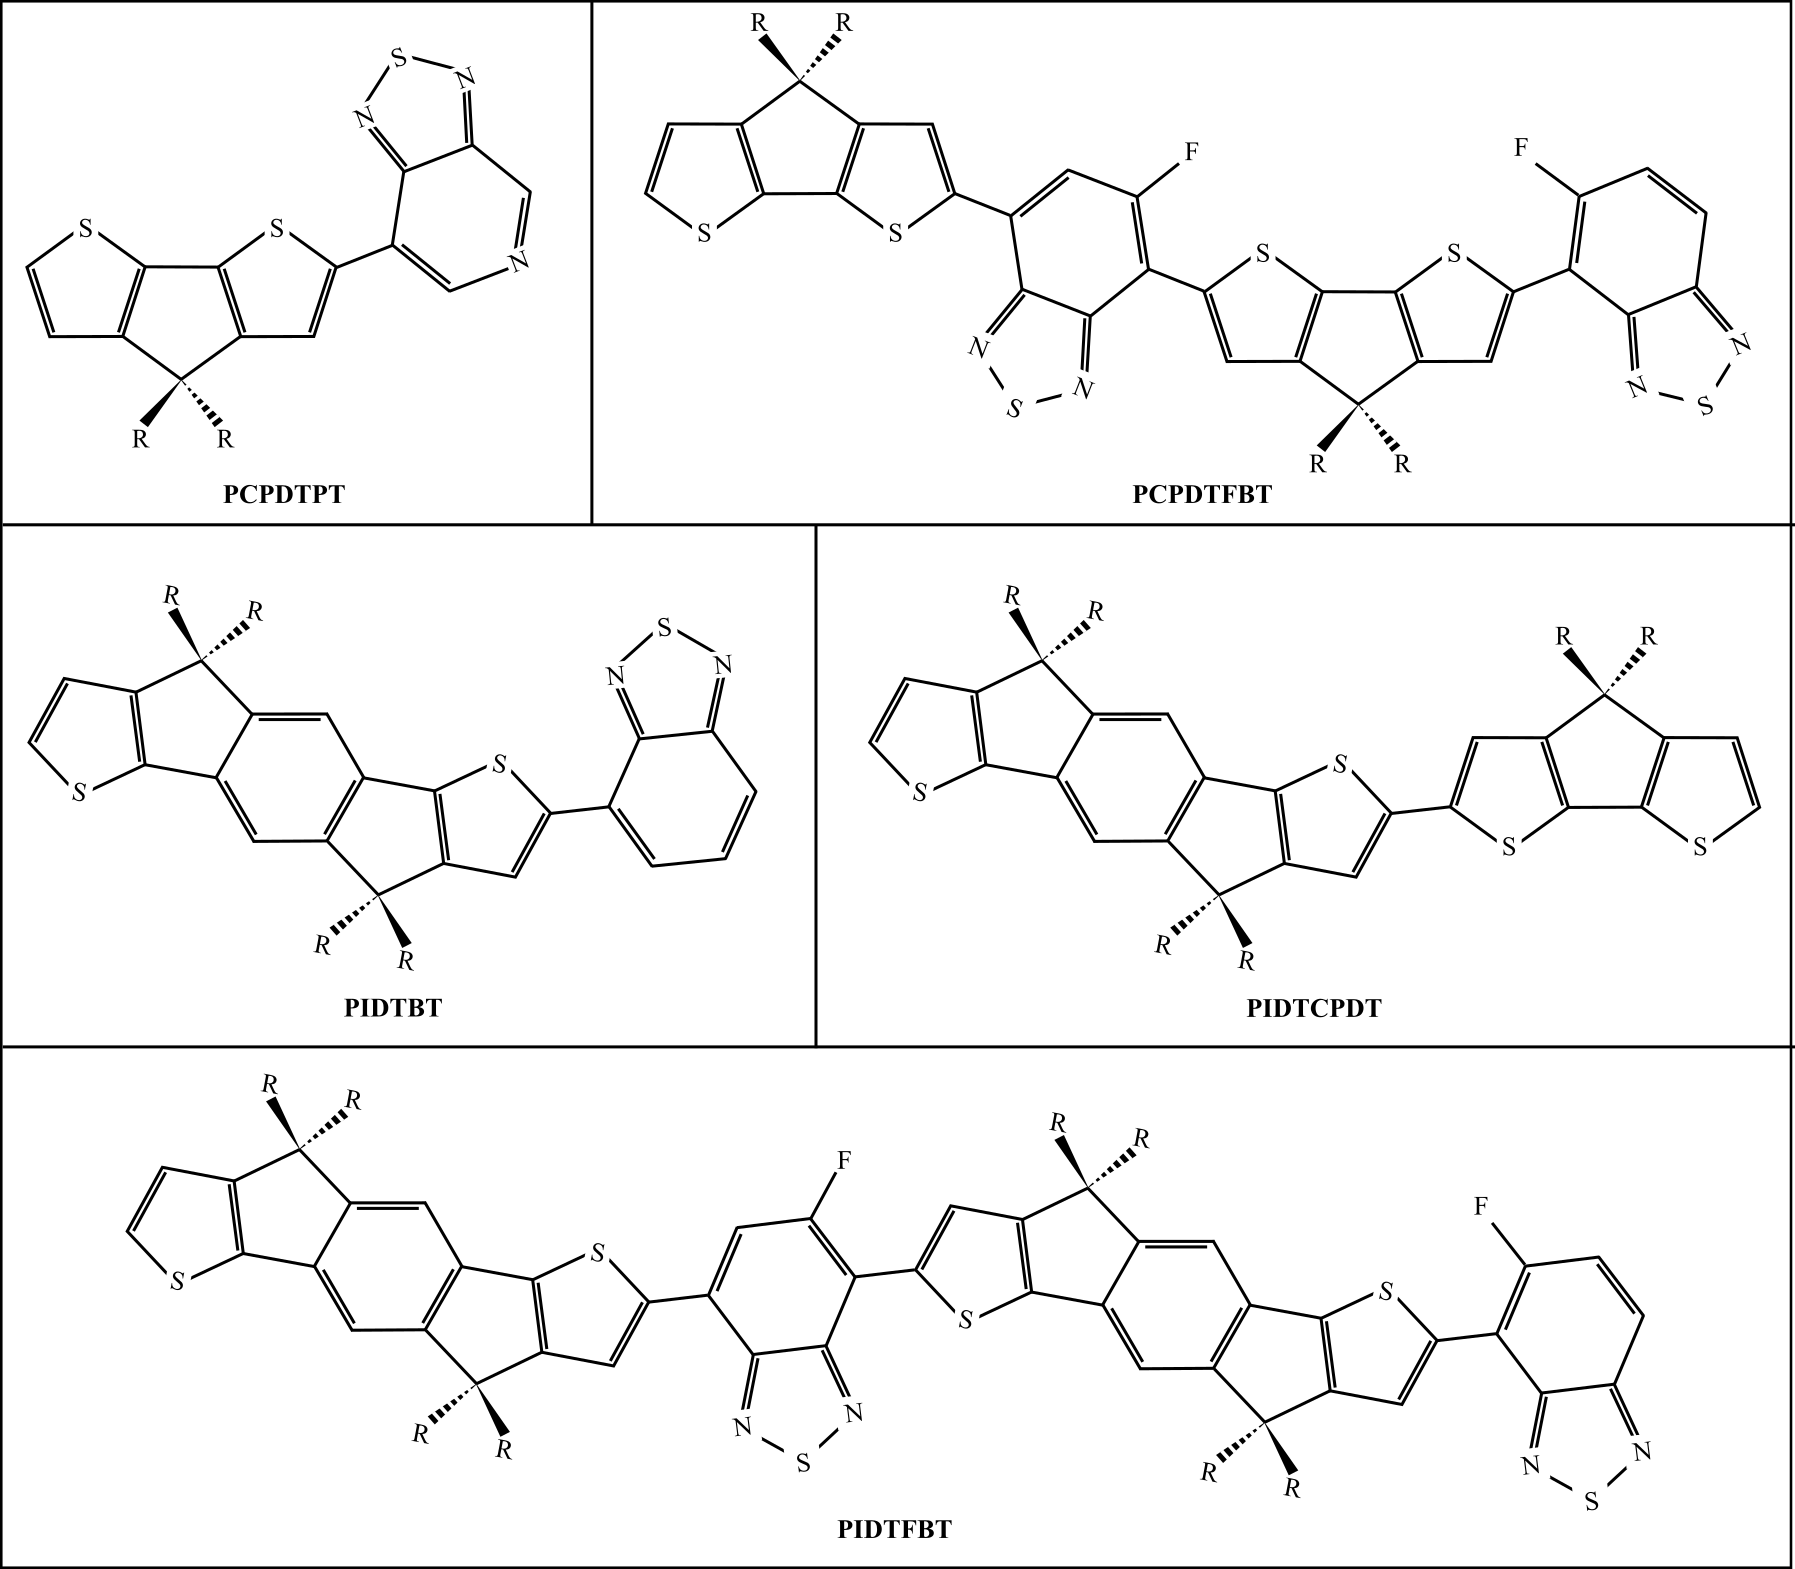
\includegraphics[width=0.9\linewidth]{src/figures/pers_l_figs/monomers.png}
    \caption{Molecular structures of the five repeating units used to build the polymers studied in this chapter. Each repeating includes a donor and acceptor region. }
    \label{fig:monomers}
\end{figure}
\newpage
\par The monomer fragments used to create the monomers in this study are cyclopentadithiophene (CPDT), pyridalthiadiazole (PT), benzothiadiazole (BT), fluorobenzothiadiazole (FBT), and indacenodithiophene (IDT). Each repeating was built to exhibit both donor and acceptor regions. \autoref{fig:monomers} depicts how the repeating units, or monomers were build from the monomer fragments listed above. The polymers with PIDTBT, PCPDTPT and PIDTCPDT backbones have an A-B-A-B polymerization pattern. PCPDTFBT and PIDTFBT polymers also consider the F functional group location, altering between a meta and an ortho position. The polymerization pattern for PIDTFBT and PCPDTFBT is A-B\textsubscript{m}-A-B\textsubscript{o}, where B\textsubscript{m} is meta-FBT and B\textsubscript{o} is ortho-FBT.  In this study, we investigate the effect of backbone chemistry as well as side chain complexity on the rigidity of the polymer, the side-chains are shown in \autoref{fig:rgroups}. Calculating the persistence length is not only a way to gain more of an understanding of polymer physics, but is also another means to validate the workflow developed in Chapter 4. 
\par We are using an implicit solvent model in this study, so we utilize temperature to mimic solvent effects, to justify this we must dive into polymer theory. We first need to define an ideal chain. An ideal chain is a model in polymer theory where monomer units along the polymer have no interactions. In a real chain, interactions would be observed between monomers as well as between the polymer and solvent. The theta temperature ($\Theta_{T}$) is the temperature at which a real polymer behaves as an ideal chain \citep{doi, rubin}. Similarly, the theta solvent ($\Theta_{S}$) is the solvent in which the polymer behaves as an ideal chain. Because we are modeling our solvent implicitly, we use the temperature to tune the ideality of our polymer chains, therefore mimicking how the solvent would effect chain behavior in experiment. We calculate the temperature at which we would expect the $l_p^{MD}$ and $l_p^{SANS}$ to match and compare this to the calculated $\Theta_{T}$ in order to draw conclusions on the solvent effects $C_6D_5Cl$ has on each polymer in the experimental data. 
\begin{figure}[h!]
    \centering
    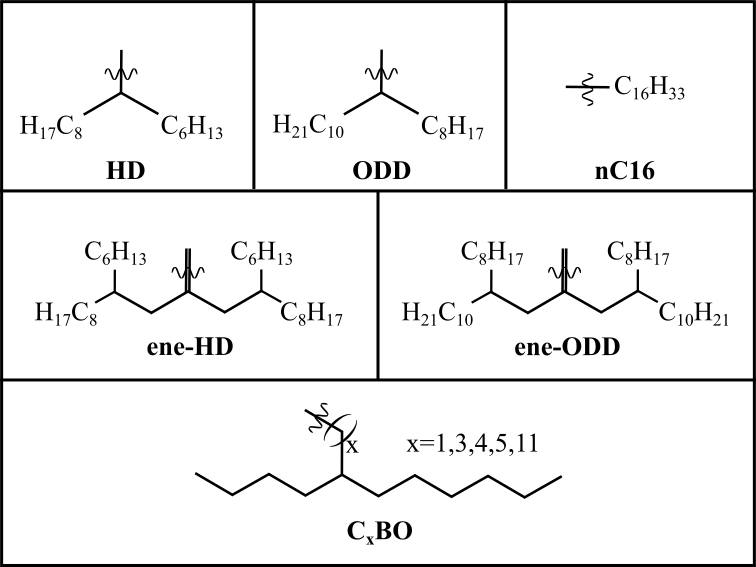
\includegraphics[width=0.8\linewidth]{src/figures/pers_l_figs/r_groups.png}
    \caption{Molecular structures of the six R-groups used as side chains in this study.}
    \label{fig:rgroups}
\end{figure}
\newpage

\section{Methods}
In this study, we conducted molecular dynamics simulations using \texttt{HOOMD-Blue} to investigate the persistence length of 13 various polymers. Simulations were performed on the Fry high performance computing cluster at Boise State using NVIDIA P100 and V100 GPUs. Each simulation was conducted in the canonical ensemble (NVT), in which the number of particles, volume, and temperature are all held constant throughout the simulation. Particle positions and velocities were updated using a two-step velocity-verlet integration of Newton’s laws of classical mechanics. The \texttt{FlowerMD} software package was utilized to construct our simulation object and initialize the simulations \citep{Albooyeh2023}. All simulations were initialized using the \texttt{Pack} functionality, in which the polymers are randomly placed in a cubic simulation box with periodic boundary conditions enforced. The simulation box size is calculated from the desired density, which is listed in \autoref{densities} for each polymer in \autoref{app:pers_len}. Thirteen conjugated polymers with similar backbone structures and varying side chain lengths were simulated in this study. An \texttt{espaloma} forcefield was generated for each polymer using the workflow outlined in Chapter 4. All simulations were run using an uncharged, united-atom model by removing the partial charges of each particle and adding the masses of the hydrogens into the neighboring, bonded atom. For each simulation we initialized a polymer of 250 monomer units in a large simulation space. Simulations were conducted at temperatures of
252, 503, 1006, 1258, 1510, 1761, 2013 K to capture how the persistence lengths evolve with temperature. The high temperatures were used to investigate how the persistence length might vary at high temperatures, but we focus on temperatures 252 K - 1006 K for analysis because temperatures above this are unrealistic for experimental settings. Simulations were run for $5 \times 10^7$ timesteps at a timestep size, dt = 0.001$\tau$. $\tau = \sqrt{M*L^2/E}$ , where M, L, and E are the reference mass, length, and energy of the simulation, respectively. From this information, the each timestep was 1.97 fs, resulting in a 98 ns simulation. 

\begin{wrapfigure}{l}{0.5\textwidth}
    \begin{center}
        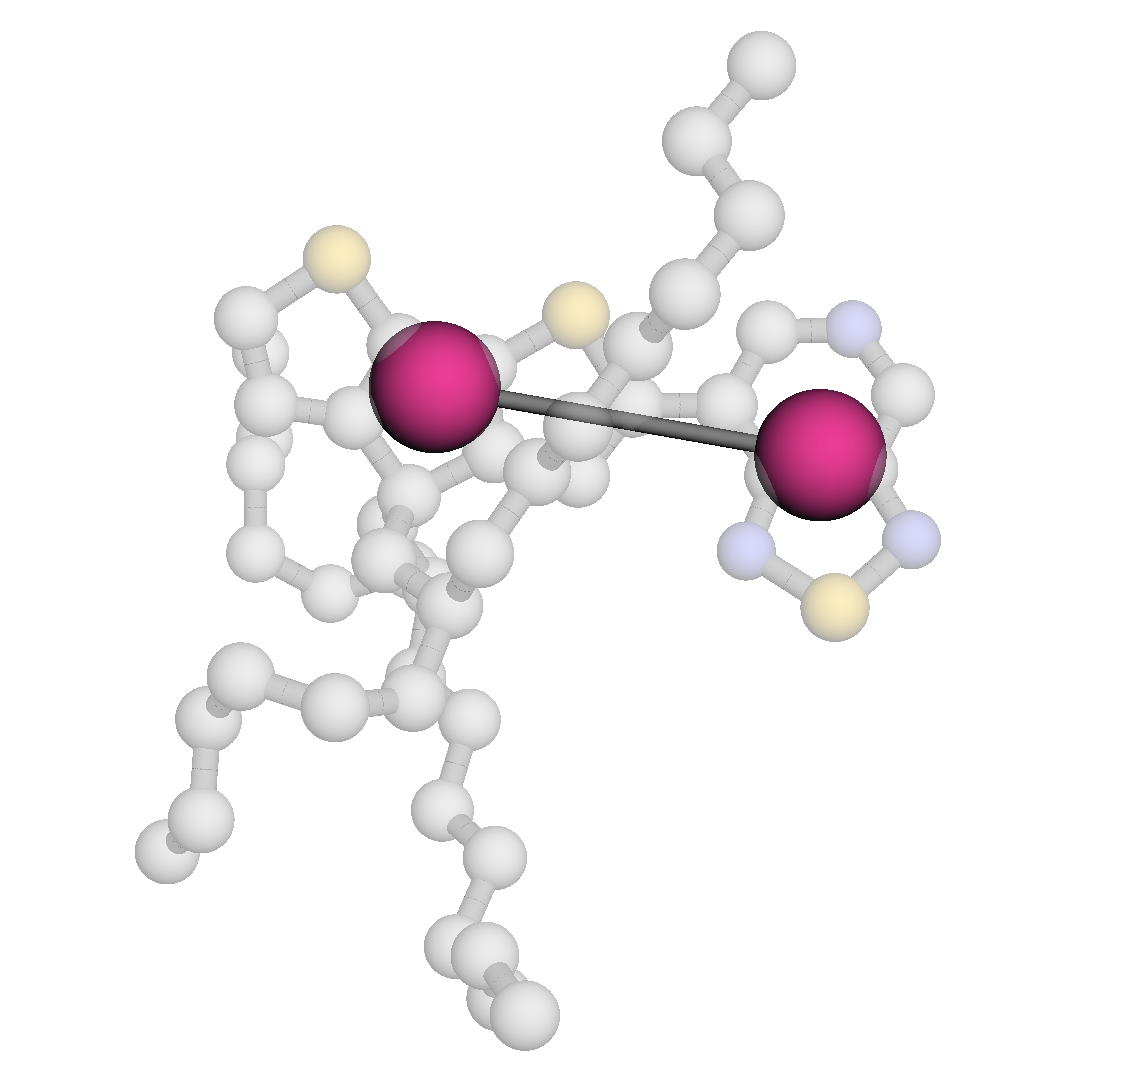
\includegraphics[width=0.48\textwidth]{src/figures/pers_l_figs/pcpdtpt_hd_cgmapping.png}
    \end{center}
  \caption{PCPDTPT-HD geometric centers used in calculating persistence length. The pink beads represent the monomer center of mass for the backbone molecules, CPDT on the left and PT on the right. The side chains were not included in the calculation of the center of mass.}
  \label{fig:CG_diagram}
\end{wrapfigure}

Once the simulations reached equilibrium and had at least 50 independent samples for each simulation the geometric center of masses were calculated using the GRiTS software \citep{grits}. This software takes an input of either the SMILES string for the portion of the molecule that you are replacing with a bead or the indices that should be replaced by a bead. In this study we used particle indices to manually determine where the beads should be placed rather than using SMILES string matching. In \autoref{fig:CG_diagram} we show an example of how a PCPDTPT-HD monomer's center of mass was calculated and where the sphere was placed. The beads are placed at the center of mass of the input indices provided by the user. The geometric centers were calculatedly adding a bead to each fully-rotatable unit to ensure that no sensitivity was lost in the persistence length calculation. 
The persistence length is determined to be the polymer length between the first monomer in the polymer chain and the first fully decorrelated monomer unit. A depiction of this is shown in \autoref{pers_length}. 
For this study, the persistence length was calculated by determining how each geometric center bead in the polymer correlates to the first bead at index 0. The correlation function ($C(n)$) is shown in \autoref{C_n1}. This equation explains how the angle correlation of the $n$\textsuperscript{th} bead is equal to the averaged dot products of the first bond vector ($\hat{a_{0}}$) and the $n$\textsuperscript{th} bond vector ($\hat{a_{0+n}}$). 
\begin{eqnarray}
  &&C(n) = \langle \cos{\theta_{0,0+n}} \rangle = \langle \hat{a_{0}} \cdot \hat{a_{0+n}} \rangle
  \label{C_n1}
\end{eqnarray}
The exponential relationship of the C(n) and n is shown in \autoref{C_n2}. The exponential coefficient of the autocorrelation function can be used to determine the persistence length, $l_p$ from the average bond lenght, $l_{b}$. 
\begin{eqnarray}
  &&C(n) \approx  \exp{\left(\frac{- n l_{b}}{l_{p}}\right)}  \approx \langle \hat{a_{0}} \cdot \hat{a_{0+n}} \rangle
  \label{C_n2}
\end{eqnarray}
Using these relationships, a python function was written to calculate $l_p$ of a polymer from the predicted morphology. In this function the autocorrelation of the bond vectors in the polymer backbone was calculated for 50 independent samples. The autocorrelation of each decorrelated snapshot was fit using the \texttt{curve\_fit function} in \texttt{SciPy's Optimize module} \citep{2020SciPy-NMeth}. Using the average bond length of the backbone bonds and the exponential coefficient gained from fitting the autocorrelation function to an exponential decay, the $l_p$ was calculated using the relationship in \autoref{C_n2}. The $l_p$'s for each snapshot were then averaged together and the standard deviations were calculated using \texttt{NumPy's Statistics module} \citep{numpy}. The full script for the persistence length function can be found at github.com/madilynpaul/persistence\_length as well as in \autoref{app:pers_len}. 
By plotting the root mean square end-to-end distance, $\sqrt{\langle R^2\rangle}$, versus the temperature of the simulation we were able to calculate the approximate theta temperature of each polymer. This was accomplished by determining the length at which the polymer will behave as an ideal chain, \autoref{e-e}. 
\begin{equation}
    \langle R^2 \rangle = N_{b}{l_b}^2
    \label{e-e}
\end{equation}
We then calculated the $\sqrt{\langle R^2\rangle}$ by taking the normalization of the end-to-end vector at each temperature and, using a linear regression, calculated the temperature at which the root mean square end-to-end distance was equivalent to $\sqrt{N_b}*{l_b}^2$, where $N_b$ is the number of bonds in the polymer and $l_b$ is the average bond length. The $\sqrt{\langle R^2\rangle}$ vs T plots can be found in \autoref{app:pers_len}. 
\section{Results and Discussion}
\begin{figure}[b]
    \centering
    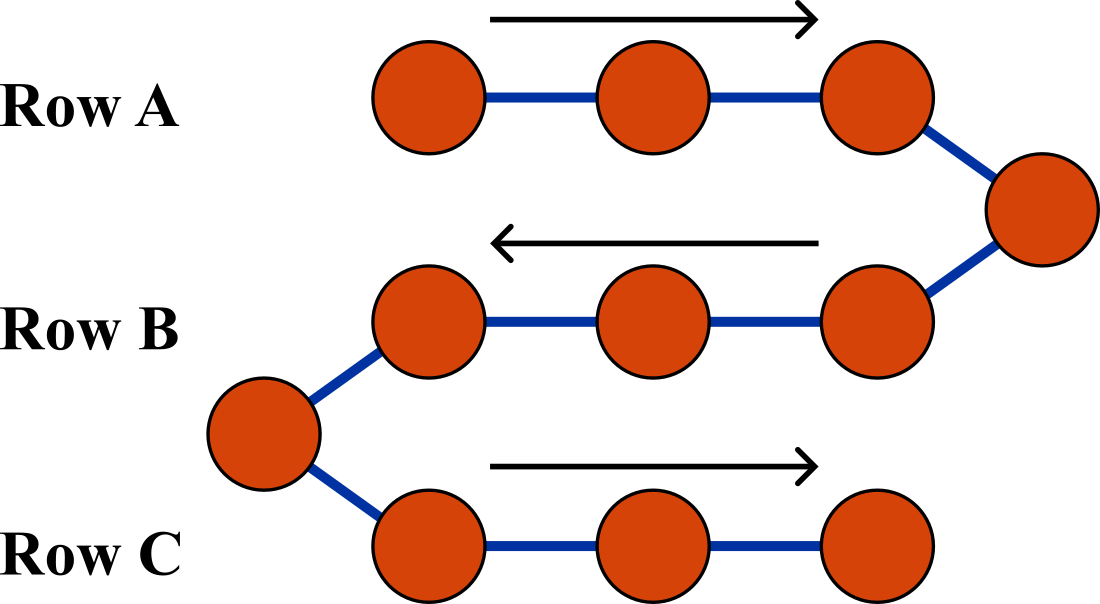
\includegraphics[width=0.5\linewidth]{src/figures/pers_l_figs/condensed_polymer.png}
    \caption{Diagram of a condensed polymer. Row A, B and C show the directions of the bond vectors. A snapshot of a condensed PCPDTPT-HD polymer can be found at \autoref{fig:real_cond_polymer}.}
    \label{fig:cond_polymer}
\end{figure}
We have successfully simulated 13 polymers with proven OPV properties. Each polymer consisted of 250 repeating units and was simulated in a large volume with no other molecules present. For most polymers we see an increase in persistence length as the temperature increases, until we reach a plateau in persistence length around 1000 K. This trend is expected, at lower temperatures we observe the polymers condensing and folding in on themselves (\autoref{fig:cond_polymer}), decreasing the persistence length. At temperatures above 1000 K the polymer has so much thermal energy it can easily overcome the steric hindrances leading to a more flexible polymer. 
\subsection{PCPDTPT Backbone}
The $l_p^{MD}$'s for polymers with a cyclopentadithiophene-co-pyridalthiadiazole (PCPDTPT) backbone (\autoref{fig:monomers}) are shown in \autoref{tab:lp_pcpdtpt}. The lower $l_p^{MD}$'s observed at lower temperatures is expected and can be explained using the diagram in \autoref{fig:cond_polymer}. When the polymer condenses on itself the $l_p$ decreases and non-bonded interactions between rows of the polymer (Rows A, B, and C ) become more prevalent. We observe good alignment between the $l_p^{MD}$'s calculated over this temperature range and the $l_p^{SANS}$'s calculated at room temperature. While we observe reasonable $l_p$ values, we do not observe the same trend in $l_p$ with increasing side chain size/complexity as the  $l_p^{SANS}$. The strong non-bonded interactions between side chains observed at low temperatures lead us to believe that having more than one polymer in the simulation is necessary for properly observing the side chain effects on backbone rigidity. 

\begin{table}[ht]
    \centering
    \begin{tabular}{c|c|c|c|c}
                        &  \multicolumn{4}{c}{\textbf{l\textsubscript{p}}}  \\
        \hline
        \textbf{Polymer}  & \textbf{252 K}& \textbf{503 K}& \textbf{1006 K}& \textbf{SANS}\\
        \hline
        PCPDTPT-ene-HD    &   $39.8 \pm 1.4$&	$48.4 \pm 1.2$&   $110.7 \pm 28$&    76.6   \\
        PCPDTPT-ene-ODD   &   $21.9 \pm 0.1$&	$38.5 \pm 1.1$&   $97.8 \pm 26$&    83.4   \\
        PCPDTPT-HD        &   $36.8 \pm 0.3$&	$55.3 \pm 9.3$&   $100.4 \pm 22$&    47.3   \\
        PCPDTPT-nC16      &   $40.2 \pm 0.7$&	$60.3 \pm 1.4$&   $96.0 \pm  22$&    61     \\
        PCPDTPT-ODD       &   $56.4 \pm 1.1$&	$63.6 \pm 2.6$&   $99.6 \pm 34$&    54.9   \\
    \end{tabular}
    \caption{Persistence lengths calculated from MD predicted morphologies ($l_p^{MD}$)  of polymers with a PCPDTPT backbone in comparison to persistence lengths calculated from SANS data ($l_p^{SANS}$). All $l_p$ presented in units of \AA.}
    \label{tab:lp_pcpdtpt}
\end{table}
By fitting the $l_p^{MD}$ with a linear regression we can predict what simulation temperature would give similar results to the SANS data. These linear regressions can be found in \autoref{app:pers_len}. Due to solvent effects we expect the $l_p^{SANS}$ values to align with different temperatures for each polymer. The simulation temperature at which we can predict similar $l_p^{MD}$ values to the $l_p^{SANS}$ values were predicted using a linear regression and can be found in \autoref{tab:sanT_pcpdtpt}. The backbone rigidity and temperature effects are not the only properties that can influence the persistence length. We can draw a connection between the solvent efficiency and the $l_p$. If the $T_{SANS}$ values are greater than the $\Theta_T$ we can conclude that the experimental solvent ($C_{6}D_{5}Cl$) is a good solvent for the given polymer. $C_{6}D_{5}Cl$ appears to be a good solvent for PCPDTPT-ene-HD, PCPDTPT-ene-ODD and PCPDTPT-n-C16, while it is a less than ideal solvent for PCPDTPT-HD and PCPDTPT-ODD. This comparison can be justified in the same manor that we explain the temperature effects on a polymer. If the polymer is solvated in a poor solvent it will condense into itself, and if it is a good solvent for the polymer we can expect that the polymer will extend into the solvent.
\begin{table}[ht]
    \centering
    \begin{tabular}{c|c|c|c}
    \textbf{Polymer}   &    \textbf{$T_{SANS}$} (K) &$\Theta_T$ (K) & $\textbf{$T_{SANS}$}/\Theta_T$\\
    \hline
    PCPDTPT-ene-HD     &    692 &502.5 & 1.38             \\
    PCPDTPT-ene-ODD    &    885 &456.2 & 1.94             \\
    PCPDTPT-HD         &    389 &507.0 & 0.767             \\
    PCPDTPT-nC16       &    526 &488.3 & 1.08             \\
    PCPDTPT-ODD        &    278 &450.5 & 0.616             \\
    \end{tabular}
    \caption{Predicted simulation temperature at which $l_p^{MD}$ would match $l_p^{SANS}$ for polymers with PCPDTPT backbone. $T_{SANS}$ calculated via linear regressions shown in \autoref{app:pers_len}. $T_{SANS}$ reported in units of K.}
    \label{tab:sanT_pcpdtpt}
\end{table}

\subsection{PCPDTFBT Backbone}
\par We observe similar trends in $l_p^{MD}$ with temperature as seen in the polymers with PCPDTPT backbones as we do with cyclopentadithiophene-co- fluorobenzothiadiazole (PCPDTFBT) backbone polymers. In PCPDTFBT-C1-BO, however, we observe a higher $l_p^{MD}$ at 503 K than at 1006 K. When calculating the $l_p$ by fitting the autocorrelation to an exponential function we don't take into account the bond vectors that may be aligned with the initial bond vector, but that shouldn't be contributing to the persistence length. This is a correction that would need to be accounted for in future calculations. The uncertainty at 1006 K is large enough to incorporate the $l_p^{MD}$ at 503 K, statistically stating that the the values are essentially equal. 
\begin{table}[ht]
    \centering
    \begin{tabular}{c|c|c|c|c}
                        &  \multicolumn{4}{c}{\textbf{l\textsubscript{p}}}  \\
        \hline
        \textbf{Polymer}  & \textbf{252 K}& \textbf{503 K}& \textbf{1006 K}& \textbf{SANS}\\
        \hline
        PCPDTFBT-C1-BO    &   $37.8 \pm 0.5$    &	$115.3 \pm 1.9$   &   $99.7 \pm 21$&    67	 \\
        PCPDTFBT-C3-BO    &   $47.5 \pm 0.4$    &	$57.6 \pm 2.8$    &   $98.9  \pm 22$&    78.4   \\
        PCPDTFBT-C4-BO    &   $46.3 \pm 1.1$    &	$65.8 \pm 3.1$    &   $105.1 \pm 20$&    86.4   \\
        PCPDTFBT-C5-BO    &   $35.4 \pm 0.3$    &	$68.7\pm 1.9$     &   $104.3 \pm 28$&    114	 \\
        PCPDTFBT-C11-BO   &   $34.6 \pm 0.2$    &	$55.9 \pm 2.6$    &   $104.0 \pm 26$&    291	 \\
    \end{tabular}
    \caption{Persistence lengths calculated from MD predicted morphologies ($l_p^{MD}$)  of polymers with a PCPDTFBT backbone in comparison to persistence lengths calculated from SANS data ($l_p^{SANS}$). All $l_p$ presented in units of \AA.}
    \label{tab:lp_pcpdtfbt}
\end{table}
\par The $l_p^{MD}$ values match well with the $l_p^{SANS}$ values for all polymers with the PCPDTFBT backbone besides that with the C11-BO side chain. The C11-BO side chain is much larger and bulkier than the other side chains, which could be contributing to the improper modeling. It could also be observed that PCPDTFBT-C11-BO may exhibit strong solvent interactions, in which solvent molecules would need to be present within the simulation to properly model the interactions. The fact that the polymers fold in on themselves and exhibit side chain interactions at low temperatures leads us to believe that a simulation with multiple polymers could lead to increased persistence lengths due to side chain interactions. 
\begin{table}[ht]
    \centering
    \begin{tabular}{c|c|c|c}
    \textbf{Polymer}   &    \textbf{$T_{SANS}$} (K) &$\Theta_T$ (K) & $\textbf{$T_{SANS}$}/\Theta_T$ \\
    \hline
    PCPDTFBT-C1-BO     &    326 &406.5    &      0.801   \\
    PCPDTFBT-C3-BO     &    736 &515.7    &      1.43   \\
    PCPDTFBT-C4-BO     &    767 &568.5    &      1.35    \\
    PCPDTFBT-C5-BO     &    1091 &491.9   &      2.22    \\
    PCPDTFBT-C11-BO    &    3034.7 &528.1 &      5.75       \\
    \end{tabular}
    \caption{Predicted simulation temperature at which $l_p^{MD}$ would match $l_p^{SANS}$ for polymers with PCPDTFBT backbone. $T_{SANS}$ calculated via linear regressions shown in \autoref{app:pers_len}. $T_{SANS}$ reported in units of K.}
    \label{tab:T_sans_pcpdtfbt}
\end{table}
\par The predicted simulation temperature at which the $l_p^{MD}$ and $l_p^{SANS}$ will match, $T_{SANS}$ can be found in \autoref{tab:T_sans_pcpdtfbt}, along with a comparison of the $\Theta_T$. The $T_{SANS}$ increases with increasing side chain size. $C_{6}D_{5}Cl$ appears to be a good solvent for all PCPDTFBT polymers besides PCPDTFBT-C1-BO, as $T_{SANS} < \Theta_T$. The values of $T_{SANS}$ are reasonable for all PCPDTFBT backbone polymers besides PCPDTFBT-C11-BO, with a value of 3034.7 K. In our MD model we observe a plateau in the persistence length at temperatures above 1200 K. The experimental values for persistence length of PCPDTFBT-C11-BO are larger than the greatest persistence lengths we observe. Investigations into our model as well as the model being used to fit the SANS data to calculate the persistence length are necessary in order to gain insight into the origin of these differences. 
\subsection{IDT Backbone}
The final DA co-polymers we investigated were ones with indacenodithiophene (IDT) as the donor molecule and three different acceptor molecules, CPDT, FBT, and BT. We successfully simulated these rather large co-polymers with little issues. The timesteps per second (TPS) for these simulations were significantly lower than the other polymer simulations due to the increased complexity and size of the polymer backbones. 
\begin{table}[ht]
    \centering
    \begin{tabular}{c|c|c|c|c}
                        &  \multicolumn{4}{c}{\textbf{l\textsubscript{p}}}  \\
        \hline
        \textbf{Polymer}  & \textbf{252 K}& \textbf{503 K}& \textbf{1006 K}& \textbf{SANS}\\
        \hline
        PIDTBT-nC16       &   $65.4\pm 0.2$     &	$57.8 \pm 1.6$&   $200.6 \pm 26$&    1310   \\
        PIDTCPDT-C11-BO   &   $36.0 \pm 0.2$    &	$76.4 \pm 8.7$&   $182.2 \pm 49$&    236	 \\
        PIDTFBT-C11-BO    &   $79.4 \pm 3.9$    &	$90.6 \pm 23$&  $178.4 \pm 32.7$    &    254	 \\
    \end{tabular}
    \caption{Persistence lengths calculated from MD predicted morphologies ($l_p^{MD}$)  of polymers with a IDT backbone in comparison to persistence lengths calculated from SANS data ($l_p^{SANS}$). All $l_p$ presented in units of \AA.}
    \label{tab:lp_pidt}
\end{table}
We have predicted reasonable values for $l_p^{MD}$, we observe an increase in $l_p^{MD}$ with the increase in temperature, with only one outlier of PIDTBT-nC16 at 503 K, \autoref{tab:lp_pidt}. We also observe good overlap between the $l_p^{MD}$ and $l_p^{SANS}$ for the PIDTFBT-C11-BO and PIDTCPDT-C11-BO polymers. Molecular dynamics predicts a significantly lower $l_p^{MD}$ for PIDTBT-nC16 than the presented $l_p^{SANS}$. However, the $l_p^{SANS}$ for all three of these polymers is reported as longer than the contour length ($L_c$) of the polymer in experiment. This makes the direct comparison of  $l_p^{MD}$ and $l_p^{SANS}$ ineffective. Both the experimental and DFT values presented for these three co-polymers came with some caveats, leading us to believe that the method of analysis used in calculating $l_p^{DFT}$ and $l_p^{SANS}$ breaks down with larger, more complex polymers requiring additional steps to predict the $l_p^{DFT}$. For all three IDT polymers the $l_p^{SANS}$ reported is longer than the contour length of the polymer, due to the $l_p^{SANS}$>$L_c$  fitting the $l_p^{SANS}$ into the linear regression of $l_p^{MD}$ results in very high, inaccurate $T_{sans}$ values. Again, due to the plateau observed in $l_p^{MD}$ at temperatures above 1200 K, we cannot confidently say that simulating these polymers at the $T_{SANS}$ temperature will result in $l_p^{MD} \approx l_p^{SANS}$. Further investigation into both theoretical and experiential results are necessary to draw conclusions. 
\begin{table}[ht]
    \centering
    \begin{tabular}{c|c|c|c}
    \textbf{Polymer}   &    \textbf{$T_{sans}$} (K) &$\Theta_T$ (K) & $\textbf{$T_{SANS}$}/\Theta_T$\\
    \hline
    PIDTBT-nC16        &    6785 &411.7 & 16.5             \\
    PIDTCPDT-C11-BO    &    1290 &511.1 & 2.52             \\
    PIDTFBT-C11-BO     &    1591 &405.0 & 3.93             \\
    \end{tabular}
    \caption{Predicted simulation temperature at which $l_p^{MD}$ would match $l_p^{SANS}$ for polymers with IDT backbone. $T_{SANS}$ calculated via linear regressions shown in \autoref{app:pers_len}. $T_{SANS}$ reported in units of K.}
    \label{tab:T_sans_pidt}
\end{table}
\subsection{MD vs DFT}
\begin{table}[ht]
    \centering
    \begin{tabular}{l|l|ll}
         \textbf{Polymer} & \textbf{$l_p^{DFT}$}& \textbf{$l_p^{MD}$} &\textbf{$l_p^{SANS}$}\\
         \hline
         PCPDTFBT-C1-BO     & 71.1              &   $99.7  \pm 21$ &67\\
         PCPDTFBT-C3-BO     & 71.1              &   $98.9  \pm 22$ &78.4   \\
         PCPDTFBT-C4-BO     & 71.1              &   $105.1 \pm 20$ &86.4   \\
         PCPDTFBT-C5-BO     & 71.1              &   $104.3 \pm 28$ &114\\
         PCPDTFBT-C11-BO    & 71.1              &   $104.0 \pm 26$ &291\\
         PCPDTPT-ene-HD     & 48.0              &   $110.7 \pm 28$ &76.6   \\
         PCPDTPT-ene-ODD    & 48.0              &   $97.8 \pm 26$ &83.4   \\
         PCPDTPT-HD         & 44.9              &   $100.4 \pm 22$ &47.3   \\
         PCPDTPT-nC16       & 44.9              &   $96.0 \pm  22$ &61     \\
         PCPDTPT-ODD        & 44.9              &   $99.6 \pm 34$ &54.9   \\
         PIDTBT-nC16        & ($>$1 \(\mu\)m)   &   $200.6 \pm 26$ &1310   \\
         PIDTCPDT-C11-BO    & 224               &   $182.2 \pm 49$ &236\\
         PIDTFBT-C11-BO     & ($>$1 \(\mu\)m)   &   $178.4 \pm 33$ &254\\
    \end{tabular}
    \caption{A comparison of $l_p^{DFT}$ reported by Danielsen, et al.~ at Ref \citep{danielsen_chain_2022} to $l_p^{MD}$ calculated at a temperature of 1006 K.}
    \label{dft_lps}
\end{table}
The results reported by Danielsen, et al.~ for $l_p^{DFT}$ are presented in \autoref{dft_lps} as well at the $l_p^{MD}$ and the $l_p^{SANS}$ \citep{danielsen_chain_2022}. Dihedral potentials were calculated using optimized scans of the central dihedral angle ($\phi$) of each monomer unit \citep{milner}. To minimize computational cost monomer units were utilized rather than polymers and side chains were replaced by methyl groups. A numerical average of backbone conformations was estimated from a set of dihedral angles, from this the $l_p^{DFT}$ was approximated. In the DFT approach accuracy is lost in modeling all side chains as methyl groups and only modeling one monomer unit. The DFT approach also does not model temperature or solvents, whereas MD simulations are able to model long polymers, complex side chains as well as temperature and can be easily modified to model explicit solvents. 

\section{Conclusions}
The molecular dynamics approach presented here has a significantly lower computational cost, allowing for the simulation of long oligomers with full side chains. Both these factors add to our confidence in the accuracy of the persistence length calculations. We observe that molecular simulations can predict side-chain influences on persistence length. The calculated $l_p^{MD}$ show good agreement to the $l_p^{SANS}$ for the majority of the polymers in this study in terms of magnitudes and trends. From this information we can conclude that the MD workflow presented in Chapter 4 is accurately predicting bulk morphologies of DA-polymers. From this work we conclude that $l_p$ is a relatively simple measure of the thermodynamic stability of a polymer as well as a prediction of the bulk morphology and we present a MD workflow that accurately predicts and calculates the $l_p$ of DA co-polymers. 